%\documentclass[en,hazy,blue,screen,14pt]{elegantnote}
\documentclass[en,hazy,blue]{elegantnote}
\usepackage[T1]{fontenc}
\usepackage[latin9]{inputenc}
% \usepackage[USenglish]{babel}
\usepackage{babel}
\usepackage{float}
\usepackage{textcomp}
\usepackage{amsmath,amsfonts,amssymb}
\usepackage{amsthm}
\usepackage{graphicx}
\usepackage[ruled,vlined]{algorithm2e}
\PassOptionsToPackage{normalem}{ulem}
\usepackage{ulem}
\usepackage{mathtools}
\usepackage{url}
\usepackage{hyperref}
\usepackage{listings}

%%%%%%%%%%%%%%%%%%%%%%%%%%%%%%%%%%%%%%%
% Math Symbols
%%%%%%%%%%%%%%%%%%%%%%%%%%%%%%%%%%%%%%%
\renewcommand{\>}{{\rightarrow}}
\renewcommand{\hat}{\widehat}
\renewcommand{\tilde}{\widetilde}
\newcommand{\half}{\frac{1}{2}}
%
\newcommand{\R}{{\mathbb R}}
\newcommand{\Z}{{\mathbb Z}}
\newcommand{\N}{{\mathbb N}}
\renewcommand{\P}{{\mathbf P}}
\newcommand{\E}{{\mathbf E}}
\newcommand{\Var}{{\mathbf{Var}}}
\newcommand{\I}{{\mathbf I}}
\newcommand{\1}{{\mathbf 1}}
\newcommand{\0}{{\mathbf 0}}
%%%%%%%%%%%%%%%%%%%%%%%%%%%%%%%%%%%%%%%
% Code Style
%%%%%%%%%%%%%%%%%%%%%%%%%%%%%%%%%%%%%%%
\lstset{
	numbers=left, 
	numberstyle=\small, 
	numbersep=8pt, 
	frame = single, 
	framexleftmargin=15pt,
	breaklines=true,
	columns=fullflexible
}
%%%%%%%%%%%%%%%%%%%%%%%%%%%%%%%%%%%%%%%
% Theorem
%%%%%%%%%%%%%%%%%%%%%%%%%%%%%%%%%%%%%%%
\renewcommand\qedsymbol{$\blacksquare$}
\DeclarePairedDelimiter{\ceil}{\lceil}{\rceil}
\newcommand\tab[1][1cm]{\hspace*{#1}}
\newenvironment{claim}[1]{\par\noindent\underline{Claim:}\space#1}{}
\newenvironment{claimproof}[1]{\par\noindent\underline{Proof:}\space#1}{\hfill $\blacksquare$}

%%%%%%%%%%%%%%%%%%%%%%%%%%%%%%%%%%%%%%%
% Title
%%%%%%%%%%%%%%%%%%%%%%%%%%%%%%%%%%%%%%%
\title{Class Notes: STAT 501\\ Nonparametrics \& Log-Linear Models\\ $I \times J$ Tables\\ $2 \times 2 \times k$ Tables\\ $I \times J \times K$ Tables
}
\author{Da Kuang}
\institute{University of Pennsylvania}
% \version{1.00}
\date{}

\begin{document}

\maketitle
\newpage
\tableofcontents

\newpage
\section{Basic Combinatorics}
\subsection{Permutation}
How many possible combinations are there for the computer login password if it must consist of a letter followed by a number?

If a job consist of $k$ separate tasks, the $i$-th of which can be done in $n_i$ ways, $i = 1, \cdots, k$, then the entire job can be done in $n_1 \times n_2 \times \cdots \times n_k$ ways.

\begin{definition}[Factorial]
	The factorial of a positive integer $n$ is 
	\[n! = n \times (n-1) \times (n - 2) \times \cdots \times 2 \times 1\]
	Also, we define, $0! = 1$.
\end{definition}

\begin{definition}[Permutation]
A permutation of a set of objects is an ordered arrangement of the objects.
\end{definition}

\subsection{Combination}
Order is not always meaningful, for instance the order of a hand of poker cards is actually does not matter.

\begin{definition}[Combination]
We call a collection of $r$ unordered elements a combination of size $r$. In general, the number of combinations of size $r$ from a group of $n (n \ge r \ge 0)$ objects is ${n \choose r}$.

\[{n \choose r} = \frac{n!}{(n-r)!r!} = \frac{n \times (n - 1) \times (n - r + 1)}{r!}.\]
\end{definition}

\subsection{Multinomial Coefficients}
A set of $n$ distinct items is to be divided into $I$ distinct groups of respective size $n_1$, $n_2$, $\dots$, $n_I$, where $\sum_{i=1}^{I} n_i = n$. How many different divisions are possible?

There are the following possible divisions.
\begin{align*}
	&{n \choose n_1} {n-n_1 \choose n_2}\cdots{n -n_1 -n_2 - \cdots n_{I-1} \choose n_I}\\
	=&\frac{n!}{(n-n_1)!n_1!} 
	\frac{(n-n_1)!}{(n - n_1 - n_2)!n_2!}
	\cdots
	\frac{(n - n_1 - n_2 - \cdots - n_{I-1})!}{0!n_I!}\\
	=& \frac{n!}{n_1! \cdots n_I!}
\end{align*}

\begin{definition}[Multinomial Coefficient]
	We define the multinomial coefficient as 
	\[{n \choose n_1 n_2 \cdots n_I} \equiv \frac{n!}{n_1! \cdots n_I!}\]
\end{definition}

\subsection{Multinomial Distribution}
Suppose we have $n$ independent trials, 
\begin{itemize}
	\item each trial can result in one of $I$ types of outcomes;
	\item on each trial the probabilities of the $I$ outcomes are respectively
$p_1, p_2, \cdots, p_I$;
\end{itemize}
Let $X_i$ be the total number of outcomes of type $I$ in the $n$ trials. Any particular sequence of trials giving rise to $X_1 = x_1$, $X_2 = x_2$, $\cdots$, $X_I = x_I$ occurs with probability $p_1^{x_1}p_2^{x_2} \cdots p_I^{x_I}$.

Recall that there are ${n \choose x_1x_2\cdots x_I}$ such sequences. Therefore the probability for a certain sequence happens is that
\[p(x_1, \cdots, x_I) = {n \choose x_1 x_2 \cdots x_I} p_1^{x_1}p_2^{x_2} \cdots p_I^{x_I}\]

The marginal distribution of $X_1$ is 
\[\sum_{x_2, \cdots, x_I} {n \choose x_1 x_2 \cdots x_I} p_1^{x_1}p_2^{x_2} \cdots p_I^{x_I}\]

Also, binomial distribution can be derived from multinomial distribution.
\section{$I \times J$ Table}
Suppose we have two categorical variables, $X$ and $Y$. The number of categories of $X$ is $I$ and the number of categories of $Y$ is $J$.

\begin{definition}[Contingency Table]
	A rectangular table having $I$ rows for the categories of $X$ and $J$
	columns for the categories of $Y$ has cells that display the $IJ$ possible
combinations of outcomes.
	
	Sometimes, it is also called frequency table or cross-classification table.
\end{definition}

Suppose the total number of observations $n = \sum_{i = 1}^{I} \sum_{j =1}^{J}n_{ij}$. 
\begin{figure}[H]
	\centering
	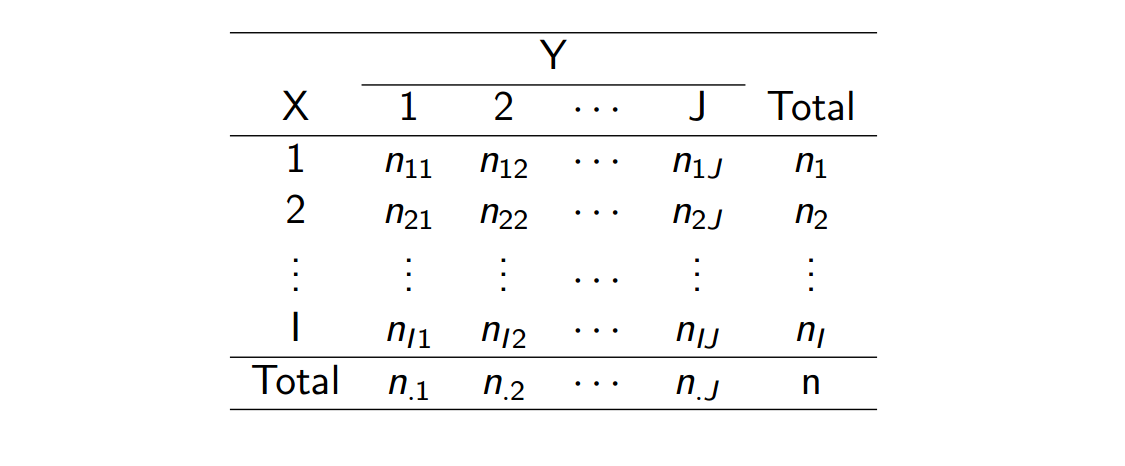
\includegraphics[width=0.7\linewidth]{fig/screenshot001}
	\caption{Example of $I \times J$ Contingency Table}
	\label{fig:screenshot001}
\end{figure}

\section{Study Designs}

\subsection{Design 1: One Multinomial Sampling with n Fixed}
If the total sample size of observations n is fixed in advance
(e.g., in a cross-sectional study), then a multinomial sampling
model might be used where cell counts are treated as
multinomial random variables with index n and probabilities $\pi_{ij}$.

\subsection{Design 2: $I$ Multinomial Distributions}
If the row totals $n_i$ are fixed in advance, the counts $n_{ij}$ have a
multinomial distribution with index $n_i$. So there are $I$ multinomial distributions.

Sometimes $n_i$ is not fixed in advance. The row variable is an explanatory variable and the column variable is a response variable. $\P(Y = j| X = i)$.

\subsection{Design 3: The Lady Tasting Tea}
If both row and column totals are fixed by design, then a
hyper-geometric sampling distribution applies for the cell counts.

\subsection{Design 4}
If observations are to be collected over a certain period of time
and cross-classified into one of the $I \times J$ categories, then a
Poisson sampling model might be used where cell counts are
treated as independent Poisson random variables with
parameters $\mu_{ij}$'s.

\section{Divide into The Fist Two Designs}
\subsection{One Multinomial Sampling with $n$ Fixed}
The contingency Table for this design is as follows
\begin{figure}[H]
	\centering
	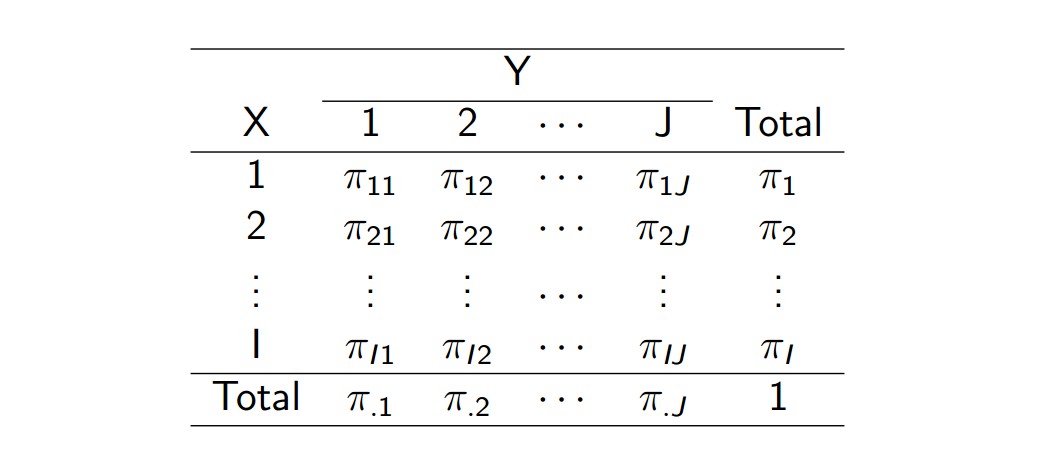
\includegraphics[width=0.7\linewidth]{fig/screenshot002}
	\caption{Example of Contingency Table}
	\label{fig:screenshot002}
\end{figure}

Here $\pi_{ij} = \P(X = i, Y = j)$ is the probability that $(X, Y)$ falls in the $ij$-th cell. The combinations of $\pi_{ij}$'s form the joint distribution of $X$ and $Y$.
\[\sum_{i=1}^{I} \sum_{j=1}^{J} \pi_{ij} = 1.\]
The marginal distribution are the row and column totals of the joint probabilities, i.e. $\pi_{i.}$'s and $\pi_{.j}$'s.
\[\P(X = i) = \pi_{i.}, \P(Y = j) = \pi_{.j}\]

Given a sequence $z_{11}, \cdots, z_{IJ}$, its coresponding probability is 
\[\P(n_{11} = z_{11}, \cdots, n_{ij} = z_{IJ}) = \frac{n!}{\prod_{i = 1}^{I} \prod_{j=1}^{J} n_{ij}!} \prod_{i=1}^{I} \prod_{j=1}^{J} \pi_{ij}^{n_{ij}}.\]

The estimator of the cell probability is $\hat{\pi}_{ij} = p_{ij} = \frac{n_{ij}}{n}$, and $\hat{\pi}_i = \frac{n_i}{n}$.

\subsection{Independence}
In this step-up, we are usually interested in the dependency between $X$ and $Y$. When $X$ does not have an effect on the probabilities for the
outcomes of $Y$, we say that $Y$ is independent of $X$.
When they are independent,
\begin{align*}
	&\P(X = i, Y = j) = \P(X = i) \P(Y =j)\\
	&\pi_{ij} = \pi_i \pi_{.j}
\end{align*}

Independence simplifies the probability structure within a
contingency table by reducing the number of unknown
parameters from $IJ$ to $I - 1 + J - 1 = I + J - 2$ marginal
probabilities.
\subsection{$I$ Multinomial Distributions}
The contingency Table for this design looks the same
\begin{figure}[H]
	\centering
	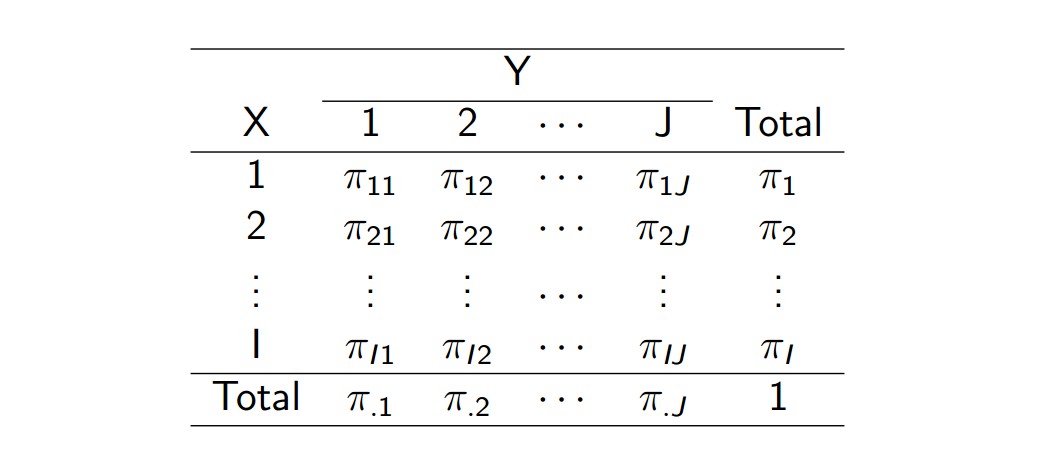
\includegraphics[width=0.7\linewidth]{fig/screenshot002}
	\caption{Example of Contingency Table}
	\label{fig:screenshot003}
\end{figure}

We have a separate $J$-category multinomial distribution in each of the $I$ groups. Define $\pi_{j|i} = \P(Y = j| X = i)$ as the probability of observing response category $j$ given that a unit is from group $i$.
\[\sum_{j= 1}^{J} \pi_{j|i} = 1, ~\text{for each } i = 1, \cdots, I.\]

The probability of observing a sequence $z_{i1}, \cdots, z_{iJ}$ from group $i$ is
\[\P(n_{i1} = z_{i1}, \cdots, n_{iJ} = z_{iJ}|n_i = \frac{n!}{\prod_{j=1}^{J} n_{ij}!} \prod_{j=1}^{J} \pi_{j|i}^{n_{ij}}\]

The full model for the contingency table is the Product Multinomial Model
\[\prod_{i=1}^{I} \frac{n!}{\prod_{j=1}^{J} n_{ij}!} \prod_{j=1}^{J} \pi_{j|i}^{n_{ij}} \]

\subsection{Independence}
Independence of $X$ and $Y$ in the context of a product multinomial
model means that the conditional probabilities for each $Y$ are equal
across the rows of the table.

For each $j = 1, \cdots J$, we have
\begin{itemize}
	\item $\P(Y = j| X = 1) = \cdots = \P(Y = j| X = I) = \P(Y = j)$.
	\item $\pi_{j|1} = \cdots = \pi_{j|I} = \pi_{.j}$
	\item $\hat{\pi}_{j|i} = \frac{n_{ij}}{n_i} = \frac{n_{ij}}{n} / \frac{n_i}{n} = \frac{\hat{pi}_{ij}}{\hat{\pi}_i}$.
\end{itemize}

Note that this condition is mathematically equivalent to
independence as defined for the one multinomial model.

\begin{proof}
	Because $X$ is not random in the product multinomial model, we
	define $\pi_i$ to be the fixed proportion of the total sample that is
	taken from group $i$.
	
	Then $\pi_{j|i} = \frac{\pi_{ij}}{\pi_i} = \pi_{.j}$
together imply that $\pi_{ij} = \pi_i \pi_{.j}$
\end{proof}

\subsection{Summary}
\begin{itemize}
	\item Parameter estimates from the one and product multinomial
	models are the same.
	\item The definitions of independence in the two models are
	equivalent.
	\item The two models lead to exactly the same conditional
	distributions for $Y$ given $X = i$.
	\item As a consequence, analyses conducted based on each model
	generally yield the same results.
	\item Therefore, when developing tests for independence and other
	analyses on contingency tables, we assume whichever model for
	the table is most convenient.
\end{itemize}
\section{Chi-squared Test of Independence}
\begin{itemize}
	\item Null Hypothesis: $X$ and $Y$ are independent.
	\item Test Statistic:
	\[T = \sum_{i=1}^{I}\sum_{j=1}^{J} \frac{(n_{ij} - \frac{n_i n_{.j}}{n})^2}{\frac{n_i n_{.j}}{n}}\]
	\item Reject the null hypothesis if 
	\[T > \chi^2_{(I-1)(J-1), 1 - \alpha}\]
\end{itemize}

\subsection{Example}
Scarlet fever is a childhood infection that among other symptoms
gives rise to severe irritation of the nose, throat and ears. 

In a study, six districts A to F were chosen. In each district,
patients were located, and parents were asked to state the site
at which they thought their child's irritation was worst.

\begin{figure}[H]
	\centering
	
\includegraphics[width=0.7\linewidth]{fig/screenshot003}
	\caption{Example of Chi-square Test}
	\label{fig:screenshot004}
\end{figure}


\lstinputlisting[language=R]{code/l11-exp2.R}

Note that there is warning when running the \texttt{chisq.test}. It is because that the chi-square test is based on CLT but the sample size is not large enough for approximation. 

To have enough sample size, for all cells of the contingency table, we have
\[\frac{n_i n_{.j}}{n} > 1 \text{ or } > 5.\]

We turn to Fisher Exact test to have better result. But note that the odd ratio is undefined for multinomial distribution.
\section{$2 \times 2 \times k$ Table}
\subsection{Setup}
The data consist of $k$ strata, $i = 1, 2, \cdots, k$. Within each stratum, we have a $2 \times 2$ table.
\begin{figure}[H]
	\centering
	
\includegraphics[width=0.7\linewidth]{fig/screenshot004}
	\caption{One of the Stratum}
	\label{fig:screenshot005}
\end{figure}
The two rows of the $2 \times 2$ table in the $i$-th stratum are viewed
as data from two independent binomial distributions.

\begin{figure}[H]
	\centering
	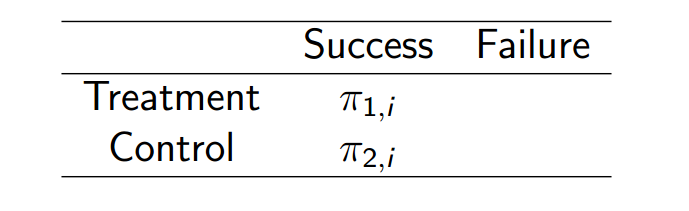
\includegraphics[width=0.5\linewidth]{fig/screenshot006}
	\caption{Probabilities in One of the Stratum}
	\label{fig:screenshot006}
\end{figure}

\subsection{Hypothesis Test}
Null hypothesis is that within each straum, the success probabilities are equal.
\[H_0: \pi_{1, i} = \pi_{2, i}, i = 1, \cdots, k.\]

Let $\theta$ denote the odds ratio for the $i$-th table.
\[\theta_i = \frac{\pi_{1, i}/ (1 - \pi_{1, i})}{\pi_{2,i}/ (1 - \pi_{2, i})}\]

Use odds ratio to represent the null hypothesis.
\[H_0: \theta_1 = \theta_2 = \cdots = \theta_k = 1\]

Note that we are testing that there is a common odds ratio and it is equal
to 1.
Moreover, $H_0$ allows for the common success probabilities to differ from
stratum to stratum.

Note that the alternative hypothesis must be consistent across the stratum. By consistent, I mean it is either
\[H_1: \pi_{1,i} \ge \pi_{2,i} \text{ for all } i = 1, \cdots, k \text{ with at least one inqeuality.}\]
or
\[H_1: \pi_{1,i} \le \pi_{2,i} \text{ for all } i = 1, \cdots, k \text{ with at least one inqeuality.}\]
\section{Mantel-Haenszel Chi-Squared Test}
In the $i$-th table, given the marginal totals $n_{1,i}$, $n_{2,i}$, $n_{.1,i}$, $n_{.2,i}$ are fixed, the random variable $n_{11,i}$ has a hyper-geometric distribution.
\[\P(n_{11,i} = z) = \frac{{n_{1,i} \choose z} {n_{2,i} \choose n_{.1,i} - x}}{{n_i \choose n_{.1,i}}}.\]

Under the $H_0$, we have
\begin{align*}
	\E (n_{11, i}) =& \frac{n_{1,i}n_{.1,i}}{n_i};\\
	\Var (n_{11,i}) =& \frac{n_{1,i}n_{2,i}n_{.1,i}n_{.2,i}}{n_i^2 (n_i - 1)}\\
\end{align*}

Also under the $H_0$, we have the statistic $\operatorname{MH}$ for Mantel-Haenszel Chi-squared Test.
\[\operatorname{MH} = \frac{\sum_{i=1}^{i}(n_{11,i} - \E (n_{11,i}))}{\sqrt{\sum_{i=1}^{i} \Var( n_{11,i})}}\]

The rejected regions are as follows.
\begin{figure}[H]
	\centering
	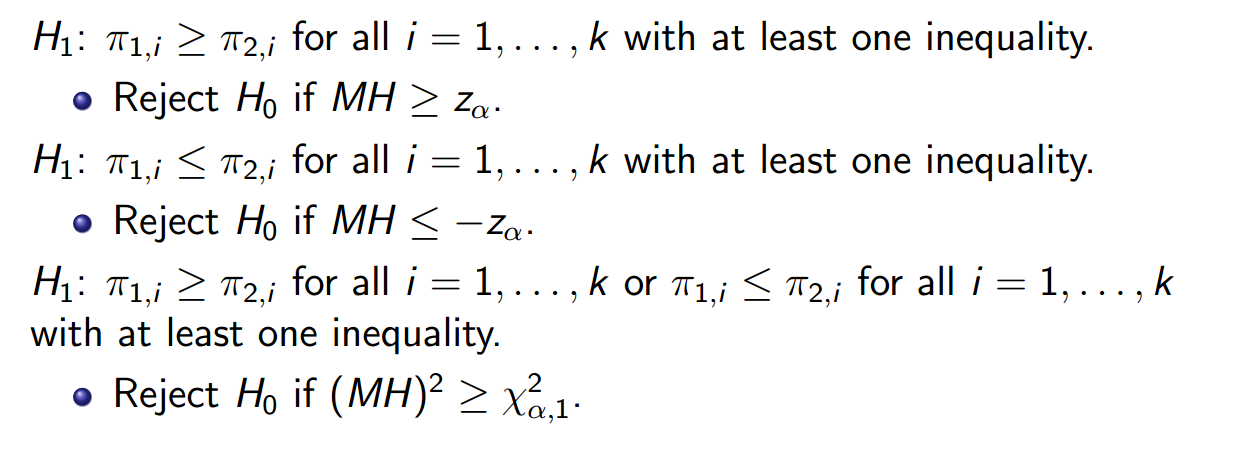
\includegraphics[width=0.7\linewidth]{fig/screenshot007}
	\caption{Rejected Region}
	\label{fig:screenshot007}
\end{figure}

\subsection{Example 1}
\lstinputlisting[language=R]{code/l11-exp3.R}

\subsection{Example 2}
Transform the data if it is not categorical.
\lstinputlisting[language=R]{code/l11-exp4.R}


\end{document}
